\documentclass[handout]{beamer}
 
\usepackage[frenchb]{babel}
\usepackage[T1]{fontenc}
\usepackage[utf8]{inputenc}
\usepackage{upgreek}
\usepackage{amsmath}
\usepackage{amssymb}
\usepackage{pdfpages}
\usepackage[]{algorithm2e}
\usepackage[abs]{overpic}
\usepackage{mdwlist}
\usepackage{tikz}
\usepackage{hhline}
\usepackage{tikz}
\usepackage{tikz-qtree}

\usetikzlibrary{trees}
\usetikzlibrary{babel}
\usetikzlibrary{arrows,automata,positioning}

\usepackage[style=alphabetic,backend=bibtex,autocite=footnote]{biblatex}

% \bibliographystyle{alpha}
\bibliography{../../articles/biblio.bib}
\nocite{*}

\usetheme{Frankfurt}
  
\title{La phylogénie des images dans les réseaux sociaux}
\author{Noé LE PHILIPPE}
\institute{Équipe ICAR - William Puech}
\date{\today}
% \logo{\includegraphics[height=10mm]{images/logo.png}}

\addtobeamertemplate{navigation symbols}{}{%
    \usebeamerfont{footline}%
    \usebeamercolor[fg]{footline}%
    \hspace{1em}%
    \insertframenumber/\inserttotalframenumber
}

\AtBeginSection[]
{
  \begin{frame}
  \frametitle{Sommaire}
  \tableofcontents[currentsection, hideothersubsections]
  \end{frame} 
}

\makeatletter
\renewcommand\@makefnmark{\hbox{\@textsuperscript{\normalfont[\@thefnmark]}}}
\renewcommand\@makefntext[1]{{\normalfont[\@thefnmark]}\enspace #1}
\makeatother

\DeclareCiteCommand{\footfullcitetext}[\mkbibfootnotetext]
{\usebibmacro{prenote}}
{\usedriver
  {\DeclareNameAlias{sortname}{default}}
  {\thefield{entrytype}}}
{\multicitedelim}
{\usebibmacro{postnote}}

\newenvironment<>{varblock}[2][.9\textwidth]{%
  \setlength{\textwidth}{#1}
  \begin{actionenv}#3%
    \def\insertblocktitle{#2}%
    \par%
    \usebeamertemplate{block begin}}
  {\par%
    \usebeamertemplate{block end}%
  \end{actionenv}}

\begin{document}

\begin{frame}
  \titlepage
\end{frame}

\section{Introduction}
\begin{frame}
  \frametitle{Le sujet de stage}

  \begin{block}{Le sujet}
    La phylogénie des images dans les réseaux sociaux
  \end{block}
  \pause
  \begin{block}{Définition}
    {\large ``La phylogenèse ou phylogénie est l'étude des relations de parenté entre êtres vivants.''}
    \hspace*\fill{\small--- Wikipedia}
  \end{block}

\end{frame}

\begin{frame}
  \frametitle{Les applications}
  \begin{block}{}
    Réduire le nombre de versions de la même image pour optimiser l'espace de stockage
  \end{block}
  \pause
  \begin{block}{}
    Suivre l'évolution et la diffusion d'images sur les réseaux sociaux
  \end{block}
  \pause
  \begin{block}{}
    Détecter l'altération d'images
  \end{block}
\end{frame}

\begin{frame}
  \frametitle{Définitions}

  \begin{block}{Near-Duplicate Image (NDI)}
    Une image I\textsubscript{n} est le near-duplicate\footnotemark\ d'une image I\textsubscript{m} si :
    $$I_{n} = T(I_{m}), T \in \mathcal{T}$$
    où $\mathcal{T}$ est un ensemble de transformations autorisées
  \end{block}\footfullcitetext{joly2007content}
  Dans le cas général, 
  \begin{multline*}
    \mathcal{T} = \{resampling, cropping, affine\ warping,\\ color\ changing, lossy\ compression\}
  \end{multline*}
  mais dans le cadre du stage, $\mathcal{T} = \{lossy\ compression\}$
\end{frame}

\begin{frame}
  \frametitle{Définitions}
  \begin{block}{Image Phylogeny Tree (IPT)}
    C'est l'arbre retraçant la parenté des images
  \end{block}

  \begin{center}
      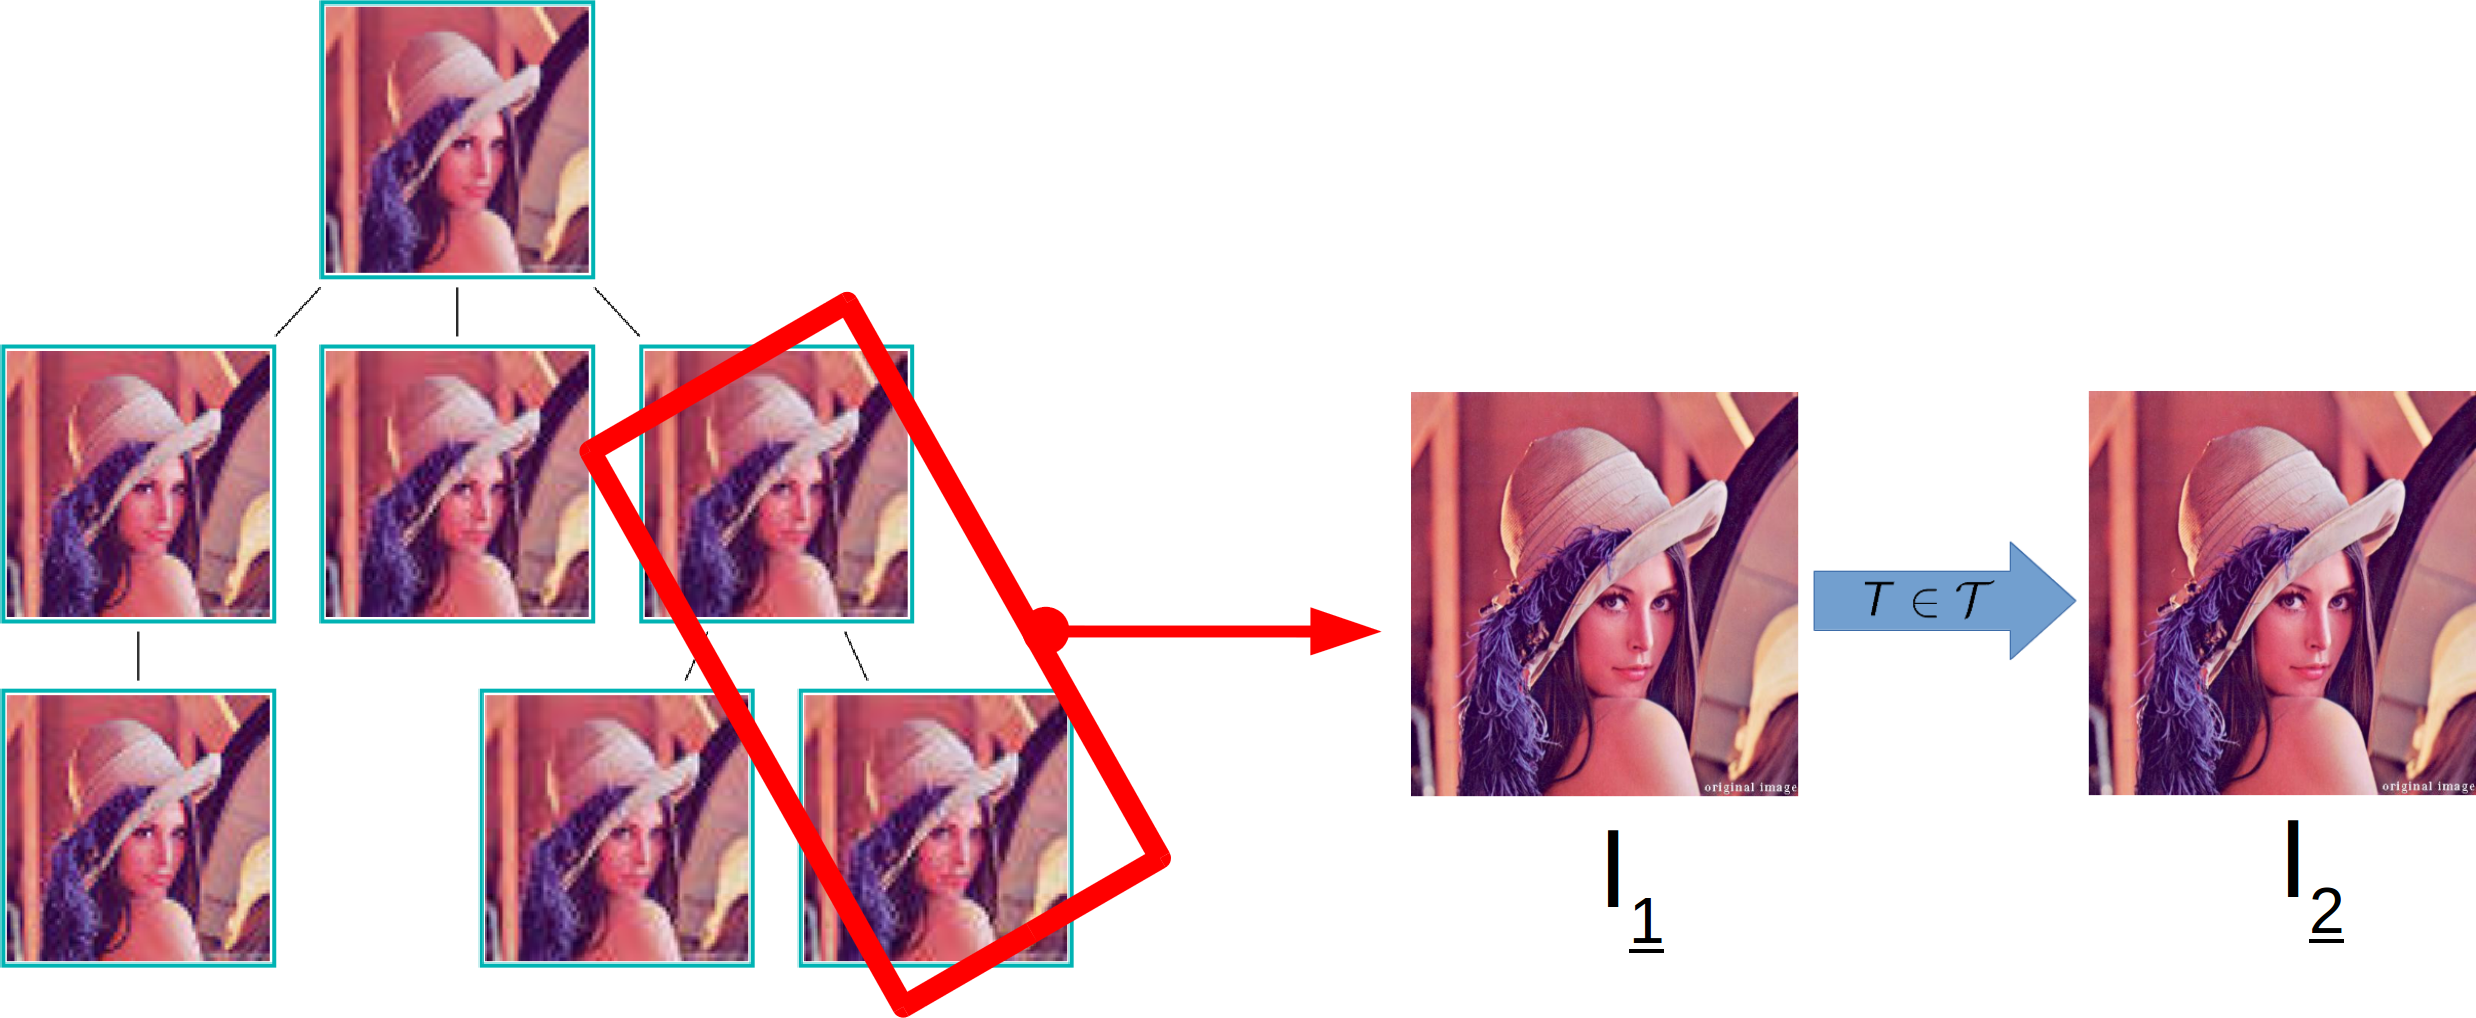
\includegraphics[width=1\textheight]{tree_extract.png}
  \end{center}

\end{frame}

\begin{frame}
  \frametitle{Image phylogeny tree}
  \begin{center}
    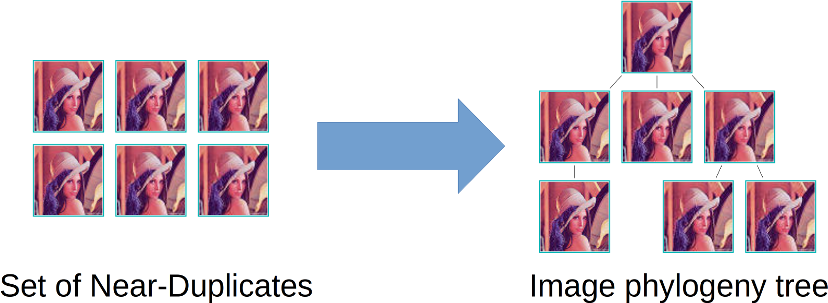
\includegraphics[width=0.8\textwidth]{set_to_tree.png}
  \end{center}
  Deux parties importantes lors de la reconstruction de l'arbre phylogénétique : 
  \pause
  \begin{columns}
    \begin{column}{0.5\textwidth}
      \begin{block}{}
        \begin{itemize}
        \item Correctement identifier la racine
        \end{itemize}
      \end{block}
      \pause
    \end{column}
    \begin{column}{0.5\textwidth}
      \begin{block}{}
        \begin{itemize}
        \item Estimer au mieux l'arborescence
        \end{itemize}
      \end{block}
    \end{column}
  \end{columns}
\end{frame}

\section{État de l'art}

\begin{frame}
  \frametitle{Estimation de l'arbre de phylogenie}

\only<1,3,5> {
  \begin{block}{Visual Migration Map}
    \begin{itemize}
    \item Les transformations sont directionnelles
    \item Relation parent-enfant si tous les détecteurs s'accordent sur la direction
    \item Simplification du graphe par sélection des plus longs chemins
    \end{itemize}
  \end{block}
  \footfullcite{kennedy2008internet}
}
  \only<2> {
    \begin{center}
      \includegraphics<2>[scale=0.3]{vmm}
    \end{center}
  }
  \only<4> {
    \begin{center}
    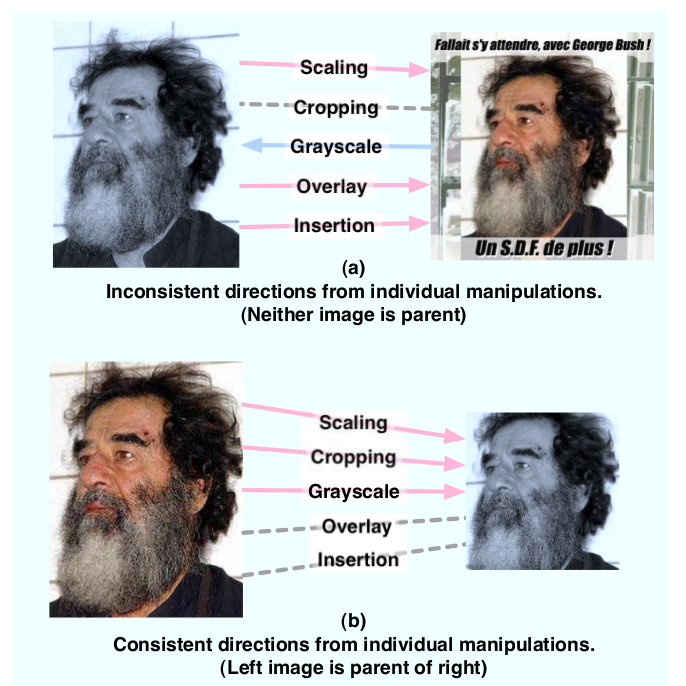
\includegraphics[scale=0.3]{vmm_directionnel}
    \end{center}
  }
  \only<6> {
    \begin{center}
    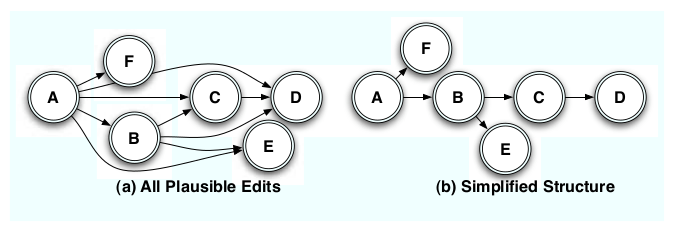
\includegraphics[scale=0.45]{vmm_tree}
    \end{center}
  }
\end{frame}

\begin{frame}
  \frametitle{Estimation de l'arbre de phylogénie}
  \begin{block}{Image phylogeny tree}
    \begin{itemize}
      \item Calcul d'une \textit{dissimilarity matrix}
      \item Calcul d'un arbre couvrant de poids min (Kruskal ou autre)
    \end{itemize}
  \end{block}
  \footfullcite{dias2010first}
  \footfullcite{dias2012image}
\end{frame}

% \section{Analyse des recompressions}
\begin{frame}
  \frametitle{Convergence des blocs lors de compressions successives}
  \begin{block}{But}
    Compter le nombre de compressions
  \end{block}
  \begin{block}{3 types de blocs}
    \begin{itemize}
      \item Les blocs plats
      \item Les blocs stables
      \item Les blocs cycliques
    \end{itemize}
  \end{block}  
  \begin{block}{Comment ?}
    plus petit commun multiple de la longueur des cycles
  \end{block}
  \footfullcite{CarneinSB2016TelltaleWatermarks}
\end{frame}

\begin{frame}
  \frametitle{Convergence des blocs lors de compressions successives}
   
    \only<1,3>{
      \begin{block}{Utilisation des blocs}
        \begin{itemize}
        \item Les blocs de l'image
        \item Insérer des blocs
        \end{itemize}
      \end{block}
      \pause
      \begin{block}{Les inconvénients}
        \begin{itemize}
        \item Nécessite du padding
        \item Limité à la même table de quantification
        \item Résultats moyens pour Q < 100
        \end{itemize}
      \end{block}  
    }

  \only<2> {
    \begin{center}
      \includegraphics<2>[scale=0.3]{insertion_blocs}
    \end{center}
  }
  \footfullcite{CarneinSB2016TelltaleWatermarks}
\end{frame}

\begin{frame}
  \frametitle{Estimation de la matrice de compression primaire}
  \only<1,3>{
    \begin{block}{Analyse des valeurs manquantes de l'histogramme}
      Artefacts distincts pour $Q^{1} > Q^{2}$ et $Q^{1} < Q^{2}$
    \end{block}
    \pause
    \begin{block}{Limites}
      \begin{itemize}
      \item $Q^{1} = Q^{2}$
      \item $Q^{1}$ est facteur de $Q^{2}$
      \end{itemize}
    \end{block}
  }
  \only<2> {
    \begin{figure}
      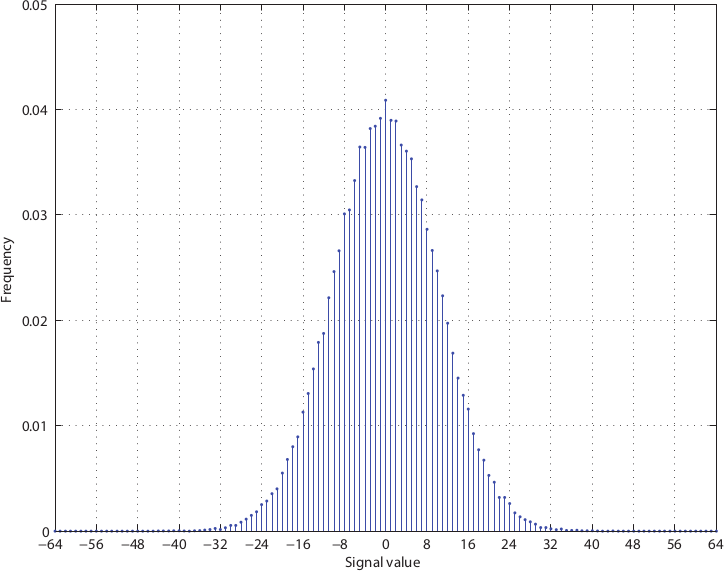
\includegraphics[height=0.4\textheight]{h1}
      \hfill
      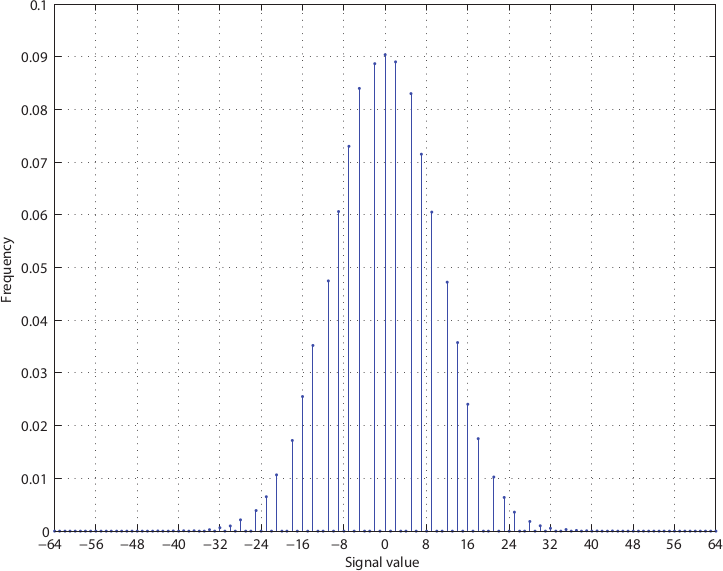
\includegraphics[height=0.4\textheight]{h2}
    \end{figure}
    \begin{figure}
      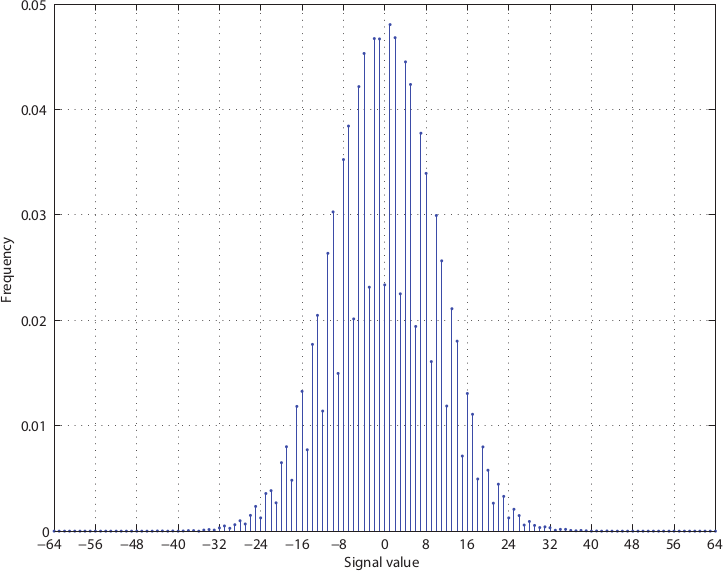
\includegraphics[height=0.4\textheight]{h3}
    \end{figure}
  }
\end{frame}

% \begin{frame}
%   \frametitle{Estimation de la matrice de compression primaire}
%   \begin{block}{Analyse des valeurs manquantes de l'histogramme}
%     Artefacts distincts pour $Q^{1} > Q^{2}$ et $Q^{1} < Q^{2}$
%   \end{block}
%   \pause
%   \begin{block}{Limites}
%     \begin{itemize}
%     \item $Q^{1} \neq Q^{2}$
%     \item $Q^{1}$ n'est pas facteur de $Q^{2}$
%     \end{itemize}
%   \end{block}
% \end{frame}

\begin{frame}
  \frametitle{Estimation de la matrice de compression primaire}
  \begin{block}{Principe de leur méthode}
    Comparer l'histogramme de l'image originale et l'histogramme des images compressées avec des tables de quantification modèles puis compressées avec $Q^{2}$ et enfin garder la table pour laquelle la différence entre histogramme est la plus faible
  \end{block}
  % \begin{enumerate}
    
  % \item Extraire la table de quantification $Q^{2}$
  %   % \end{enumerate}
  %   \suspend{enumerate}
  %   Pour tous les coefficients intéressants
  %   % \begin{enumerate}[resume]
  %   \resume{enumerate}
  % \item Obtenir l'histogramme $h_{0}$ des valeurs absolues des coefficients DCT de l'image
  % \item Crop l'image (par 4 et 4 pixels)
  % \item Sélectionner les matrices de quantification $Q^{1,1},...,Q^{1,n}$ pour chaque valeur candidate de la matrice primaire
  % \item Compresser l'image cropée avec les matrices $Q^{1,1},...,Q^{1,n}$
  % \item Décompresser toutes les images obtenue et les compresser avec $Q^{2}$

  % \end{enumerate}

\end{frame}

\section{Notre approche}
\begin{frame}
  \frametitle{Matrice de parenté}
  \begin{block}{}
    Matrice binaire de taille $n \times n$
  \end{block}
  \begin{block}{}
    Construction de l'arbre à partir de la matrice
  \end{block}
\begin{figure}
  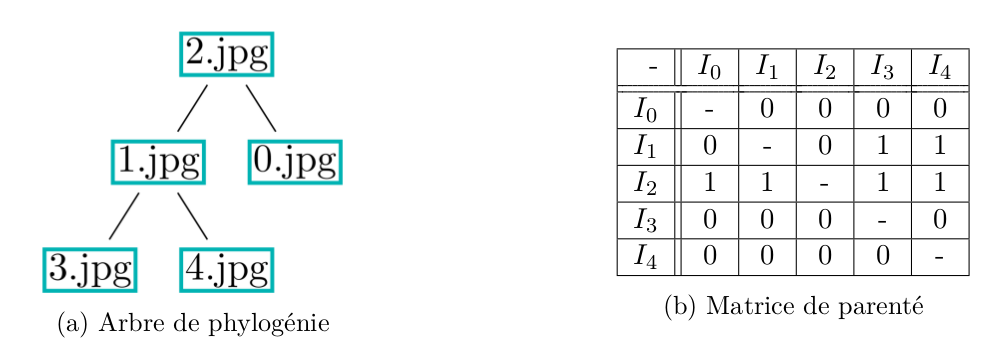
\includegraphics[width=.9\linewidth]{tree_table.png}
  % \centering
%   \subfloat[Arbre de phylogénie\label{Arbre de phylogenie}]{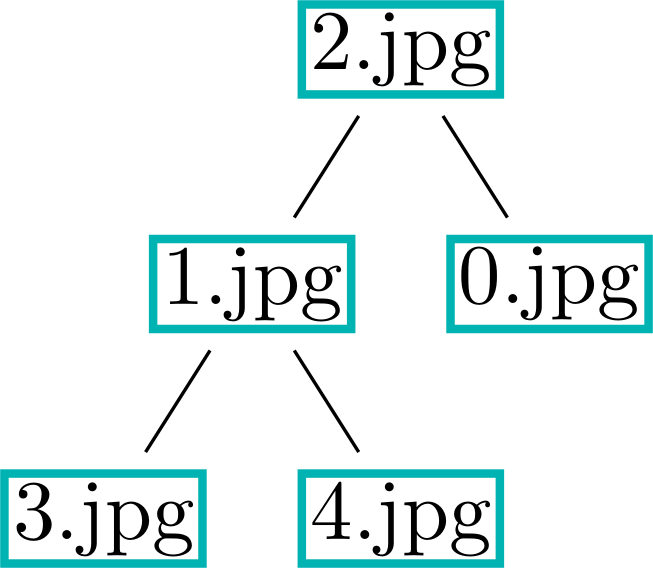
\includegraphics[width=.27\linewidth]{algo_tree.png}}
%   \subfloat[Matrice de parenté\label{fig:b}]{
%     \scalebox{0.75}{
%       \begin{tabular}{|r||c|c|c|c|c|}
%         \hline
%         - & $I_{0}$ & $I_{1}$ & $I_{2}$ & $I_{3}$ & $I_{4}$ \\ \hhline{|=::=|=|=|=|=|}
%         $I_{0}$ & - & 0 & 0 & 0 & 0 \\ \hline
%         $I_{1}$ & 0 & - & 0 & 1 & 1 \\ \hline
%         $I_{2}$ & 1 & 1 & - & 1 & 1 \\ \hline
%         $I_{3}$ & 0 & 0 & 0 & - & 0 \\ \hline
%         $I_{4}$ & 0 & 0 & 0 & 0 & - \\ \hline
%       \end{tabular} 
%     }
% }
%   \caption{A figure}
%   \label{fig:1}
\end{figure}

%   \begin{figure}
%       \centering
%       \subfloat{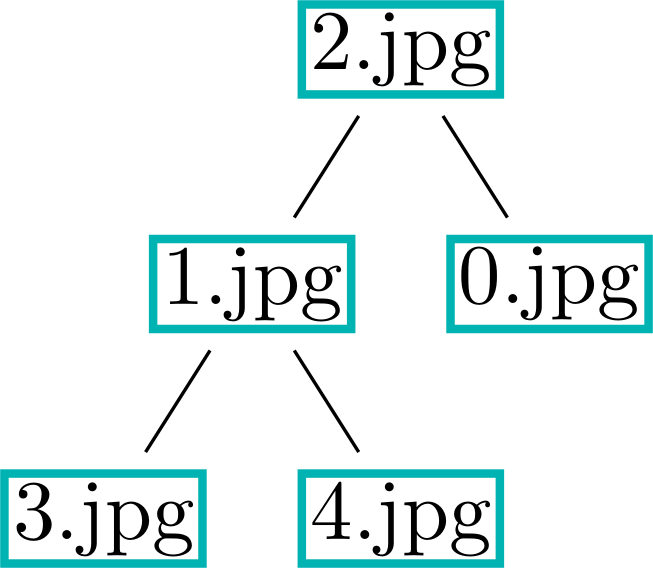
\includegraphics[width=.5\linewidth]{algo_tree.png}}
%       % \caption{Arbre de phylogénie}
%       % \label{algo_tree}
%     % \begin{subfigure}{.5\textwidth}
%       \centering
% \subfloat{
%       \begin{tabular}{|r||c|c|c|c|c|}
%         \hline
%         - & $I_{0}$ & $I_{1}$ & $I_{2}$ & $I_{3}$ & $I_{4}$ \\ \hhline{|=::=|=|=|=|=|}
%         $I_{0}$ & - & 0 & 0 & 0 & 0 \\ \hline
%         $I_{1}$ & 0 & - & 0 & 1 & 1 \\ \hline
%         $I_{2}$ & 1 & 1 & - & 1 & 1 \\ \hline
%         $I_{3}$ & 0 & 0 & 0 & - & 0 \\ \hline
%         $I_{4}$ & 0 & 0 & 0 & 0 & - \\ \hline
%       \end{tabular} 
%       % \caption{Matrice de parenté}
%       % \label{parentage_matrix}
%     % \end{subfigure}
% }
%     \caption{Une arbre de phylogénie et sa matrice de parenté.}
%     \label{parentage_tree}
%   \end{figure}

\end{frame}

\begin{frame}
  \frametitle{Notre approche}
  \begin{block}{Marqueur}
    Caractéristique de l'image qui indique qu'une certaine opération a été effectuée et qui va se transmettre aux enfants
  \end{block}
  \pause
  \begin{block}{Fonction de négation}
  $f(I_{m},I_{n})$ est une fonction qui pour tout couple d'images $(I_{m}, I_{n})$ détecte à chaque fois qu'il est présent un marqueur visible dans une image et pas dans l'autre, et donc prouve qu'il n'y a pas de relation de parenté entre $I_{m}$ et $I_{n}$.
    % $f(I_{m}, I_{n})$ est une fonction qui pour tout couple d’images (I\textsubscript{m}, I\textsubscript{n}) détecte à chaque fois qu’il est présent un marqueur indiquant qu’il n’y a pas de relation de parenté entre I\textsubscript{m} et I\textsubscript{n}.
  \end{block}
  \pause
  \begin{block}{Théorème}
  Pour tout couple d'images ($I_{m}$, $I_{n}$) d'un ensemble de near-duplicates, s'il n'existe pas de marqueur prouvant que $I_{m}$ n'est pas le parent de $I_{n}$, alors il y a une relation parent-enfant entre $I_{m}$ et $I_{n}$, $I_{m}$ $\to$ $I_{n}$.
     % Pour tout couple d'images ($I_{m}$, $I_{n}$) d'un ensemble de near-duplicates, s'il n'existe pas de marqueur prouvant que $I_{m}$ n'est pas le parent de $I_{n}$, alors il y a une relation parent-enfant entre $I_{m}$ et $I_{n}$, $I_{m}$ $\to$ $I_{n}$.
  \end{block}
  % \begin{itemize}
  % \item Tentative de preuve qu'une image n'est pas le parent d'une autre
  % \item Si c'est impossible, l'image doit alors être le parent
  % \item Extraction d'une \textit{matrice de parenté}
  % \item Calcul de l'arbre
  % \end{itemize}
  % \end{block}
\end{frame}

\begin{frame}
  \frametitle{Schéma de notre approche}
  \begin{figure}[H]
    \centering
    % \begin{tikzpicture}[auto, distance=2in,sibling distance=.25in]
    \scalebox{0.55}{
      \begin{tikzpicture}[auto,node distance=2.8cm]

        \tikzstyle{every state}=[shape=rectangle,minimum width=1.3in,text width=1.3in, align=center,fill=blue!30]
        % \tikzstyle{every data}=[shape=circle,minimum width=1.3in,text width=1.3in, align=center,fill=blue!30]

        \node[draw=none,fill=none,minimum width=1.1in,text width=1.1in, align=center] (A) {Ensemble de near-duplicates};
        \node[state] (B) [right=0.7cm of A] {DCT sur chaque image};

        \node[draw=none,fill=none,minimum width=1.1in,text width=1.1in, align=center, right=0.7cm of B] (C) {Coeffs DCT de chaque image};
        \node[state] (D) [right=0.7cm of C] {Extraction de la période de chaque coefficient DCT};

        \node[draw=none,fill=none,minimum width=1.1in,text width=1.1in, align=center, right=0.7cm of D] (E) {Tables de quantification estimées};
        \node[state] (F) [below=0.7cm of E] {Estimation du facteur de qualité};

        \node[draw=none,fill=none,minimum width=1.1in,text width=1.1in, align=center, left=0.7cm of F] (G) {$Q_f$ de chaque image};
        \node[draw=none,fill=none,minimum width=1.1in,text width=1.1in, align=center, below=0.3cm of G] (H) {Images};
        \node[state] (I) [left=0.7cm of G] {Estimation du parent};

        \node[draw=none,fill=none,minimum width=1.1in,text width=1.1in, align=center, left=0.7cm of I] (J) {Matrice de parenté};
        \node[state] (K) [left=0.7cm of J] {Construction de l'arbre};

        \node[draw=none,fill=none,minimum width=1.1in,text width=1.1in, align=center, below=1.2cm of K] (L) {Arbre non traité};
        \node[state] (M) [right=0.7cm of L] {Filtrage des doublons};
        
        \node[draw=none,fill=none,minimum width=1.1in,text width=1.1in, align=center, right=0.7 of M] (N) {Arbre de phylogénie};

        \path [->] (A) edge node[left] {} (B);
        \path [->] (B) edge node[left] {} (C);      
        \path [->] (C) edge node[left] {} (D);      
        \path [->] (D) edge node[] {} (E);      
        \path [->] (E) edge node[right] {} (F);      
        \path [->] (F) edge node[right] {} (G);      
        \path [->] (G) edge node[left] {} (I); 
        \path [->] (H) edge node[left] {} (I);
        \path [->] (I) edge node[left] {} (J);
        \path [->] (J) edge node[left] {} (K);
        \path [->] (K) edge node[left] {} (L);
        \path [->] (L) edge node[left] {} (M);
        \path [->] (M) edge node[left] {} (N);
      \end{tikzpicture}}
    % \caption{Schéma général de notre méthode.}
    \label{fig:method_schema}
  \end{figure}
\end{frame}

\begin{frame}
  \frametitle{Points clés de notre approche}
  \begin{block}{}
    Réduction d'un problème de reconstruction d'un arbre de phylogénie à un problème de négation de parenté
  \end{block}
  \begin{block}{}
    Facilement extensible
  \end{block}
\end{frame}

\begin{frame}
  \frametitle{Les marqueurs : facteur de qualité}
  \centering
  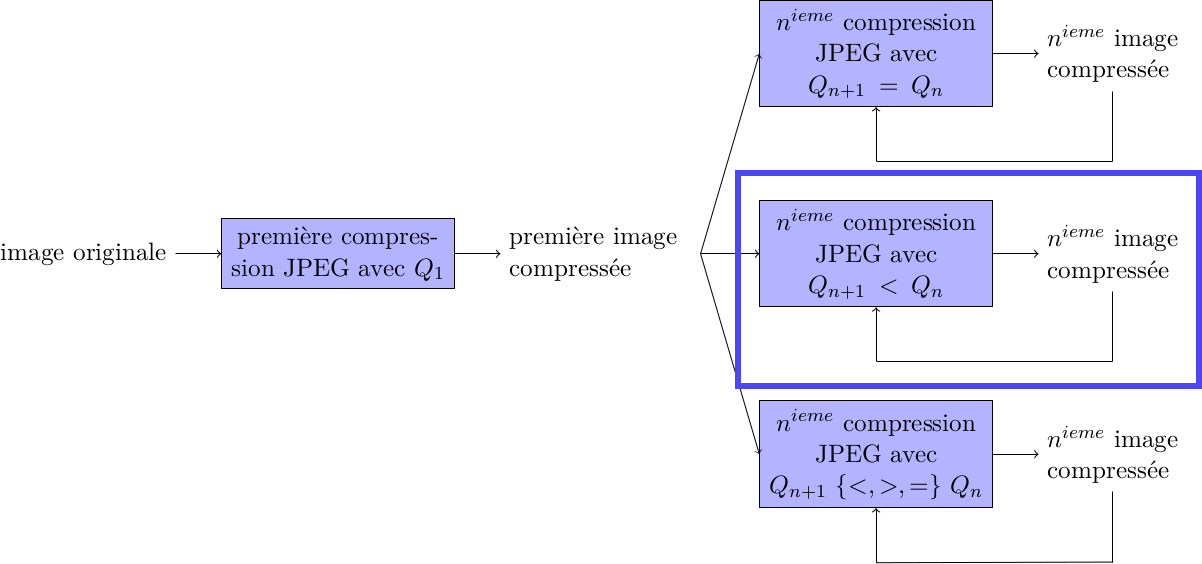
\includegraphics[width=0.8\linewidth]{qinf.png}
  \begin{block}{}
    Estimation du facteur de qualité
  \end{block}
\end{frame}

\begin{frame}
  \frametitle{Les marqueurs : valeurs manquantes dans l'histogramme des coefficients DCT}
  \begin{block}{}
    Les coefficients sont des multiples des valeurs de la table de quantification
    
  \end{block}
  \begin{figure}
    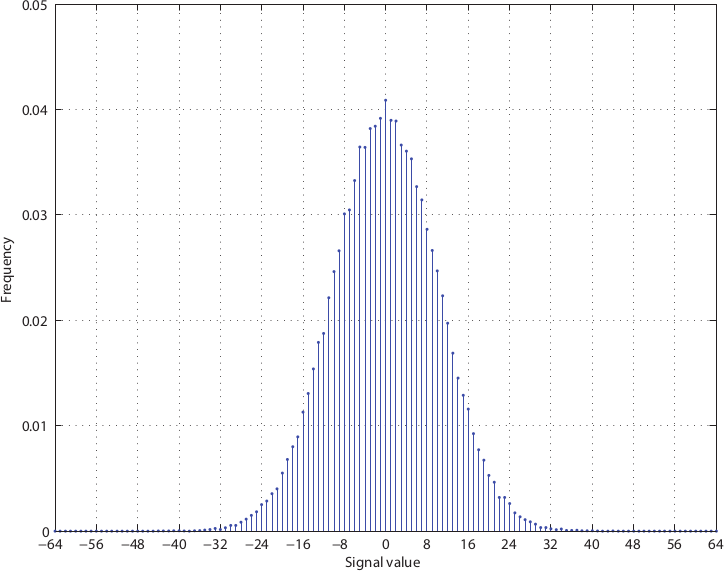
\includegraphics[width=0.5\linewidth]{h1.png}
    % \caption{Image compressée une fois}
    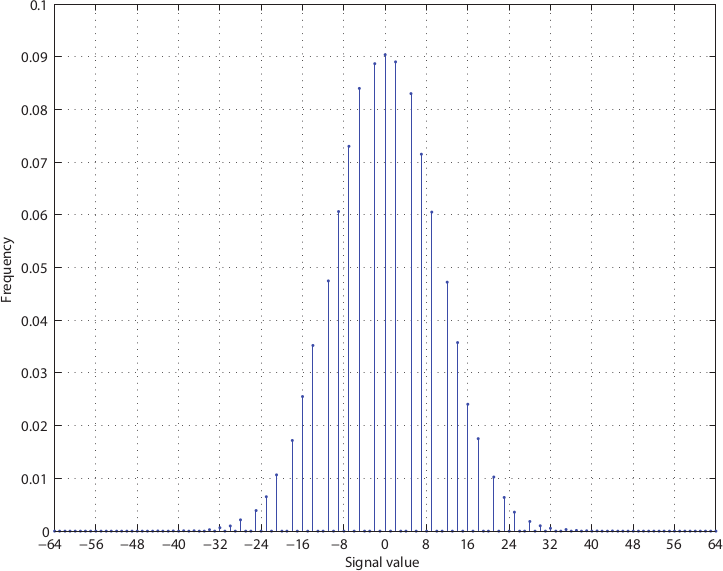
\includegraphics[width=0.5\linewidth]{h2.png}
    % \caption{\ \ Image simplement compressée - Image doublement compressée, $Q_1 > Q_2$}
  \end{figure}
\vspace{-5mm}
\scalebox{0.7}{
  \hspace{15mm}
  \textit{Image simplement compressée}
  \hspace{18mm}
  \textit{Image doublement compressée, $Q_1 > Q_2$}
}  
\end{frame}

\section{Résultats}
\begin{frame}
  \frametitle{Des résultats mitigés}
  \begin{block}{}
    Détection du parent direct très fiable
  \end{block}
  \pause
  \begin{block}{}
    Mauvaise détection des parents éloignés
  \end{block}
  \pause
  \begin{block}{}
    Arbre incomplet dans le cas d'images manquantes
  \end{block}
\end{frame}

\section{Conclusion}
\begin{frame}
 \frametitle{Conclusion - perspectives}
 \begin{block}{}
   Une méthode prometteuse
 \end{block}
 \begin{block}{}
   Trouver d'autres marqueurs
 \end{block}
 \begin{block}{}
   Traiter tous les cas de la compression JPEG
 \end{block}
 \begin{block}{}
   Ne pas se limiter à la compression
 \end{block}
\end{frame}

\begin{frame}
  \frametitle{Conclusion - perspectives}
  \centering
\scalebox{3}{
  Des questions ?
}
\end{frame}

\end{document}

